\documentclass[11pt,conference]{IEEEtran}

\usepackage{amsmath,amssymb,amsfonts}
\usepackage{algorithmic}
\usepackage{graphicx}
\usepackage{subcaption}
\usepackage{textcomp}
\usepackage{xcolor}
\usepackage[inline]{enumitem}
\newlist{inlist}{enumerate*}{1}
\setlist[inlist]{label= (\alph*)}
\usepackage[colorlinks]{hyperref}
\hypersetup{%
    colorlinks=true,
    linkcolor=blue,
    urlcolor=cyan,
    citecolor=blue
}
\usepackage[style=ieee]{biblatex}
\addbibresource{sources.bib}

\newcommand{\matlab}{MATLAB}
\newcommand{\mmatlab}{\textmu\matlab}
\newcommand{\colorlib}{CoLoR}
\renewcommand{\algorithmiccomment}[1]{\% #1}
\newcommand{\inputcoq}[1]{\InputIfFileExists{#1.v_tex}{}{\typeout{No file #1.v_tex.}}}

\begin{document}

\title{Final paper: Towards Proving Termination of \texttt{zelda-mosaic} Algorithms under Conditions on the Input}

\author{\IEEEauthorblockN{Justin Do}
\IEEEauthorblockA{\textit{Computer Science} \\
\textit{UNC Chapel Hill}\\
Chapel Hill, USA \\
\texttt{justindo@cs.unc.edu}}
\and
\IEEEauthorblockN{D. Ben Knoble}
\IEEEauthorblockA{\textit{Computer Science} \\
\textit{UNC Chapel Hill}\\
Chapel Hill, USA \\
\texttt{david3@cs.unc.edu}}
}

\maketitle

\begin{abstract}
    We report on a study of previous set of algorithms that we developed for
    building mosaics, implemented in \matlab\@. In particular, we are interested
    in the formalization of the algorithms and the relevant \matlab\ structures
    in Coq~\cite{Coq} and the termination of these algorithms under appropriate
    to-be-determined conditions. We present details on the algorithms along with
    our motivations for studying them. We then discuss an initial foray into
    related work. Next, we show an updated timeline for our progress. Lastly, we
    briefly identify the major contributions of each author to this proposal.
\end{abstract}

% \begin{IEEEkeywords}
% \end{IEEEkeywords}

\section{Summary of Proposal}

We have previously developed \texttt{zelda-mosaic}~\cite{zelda_mosaic} which
includes \matlab~\cite{matlab} code to create tiled ``mosaics'' from a set of
smaller input images. In our original proposal, we set out to prove the
termination of our mosaic-generation algorithms.

In the original work, we took a series of related images (specifically, from one
of the many ``Legend of Zelda'' ({\copyright} Nintendo) games) and automatically
stitched them together to form mosaics of game-related artwork.
\figurename~\ref{F:zelda-mosaic-sample} showcases an example output. The program
is extendable and has been successfully used on several different sizes of
inputs and for applications beyond the original project.

\begin{figure*}[pht]
    \centering
    \begin{subfigure}{0.35\textwidth}
        
\includegraphics[width=\linewidth]{img/oracleofages-original.jpg}
        \caption{Original key-art}
    \end{subfigure}
    \begin{subfigure}{0.35\textwidth}
        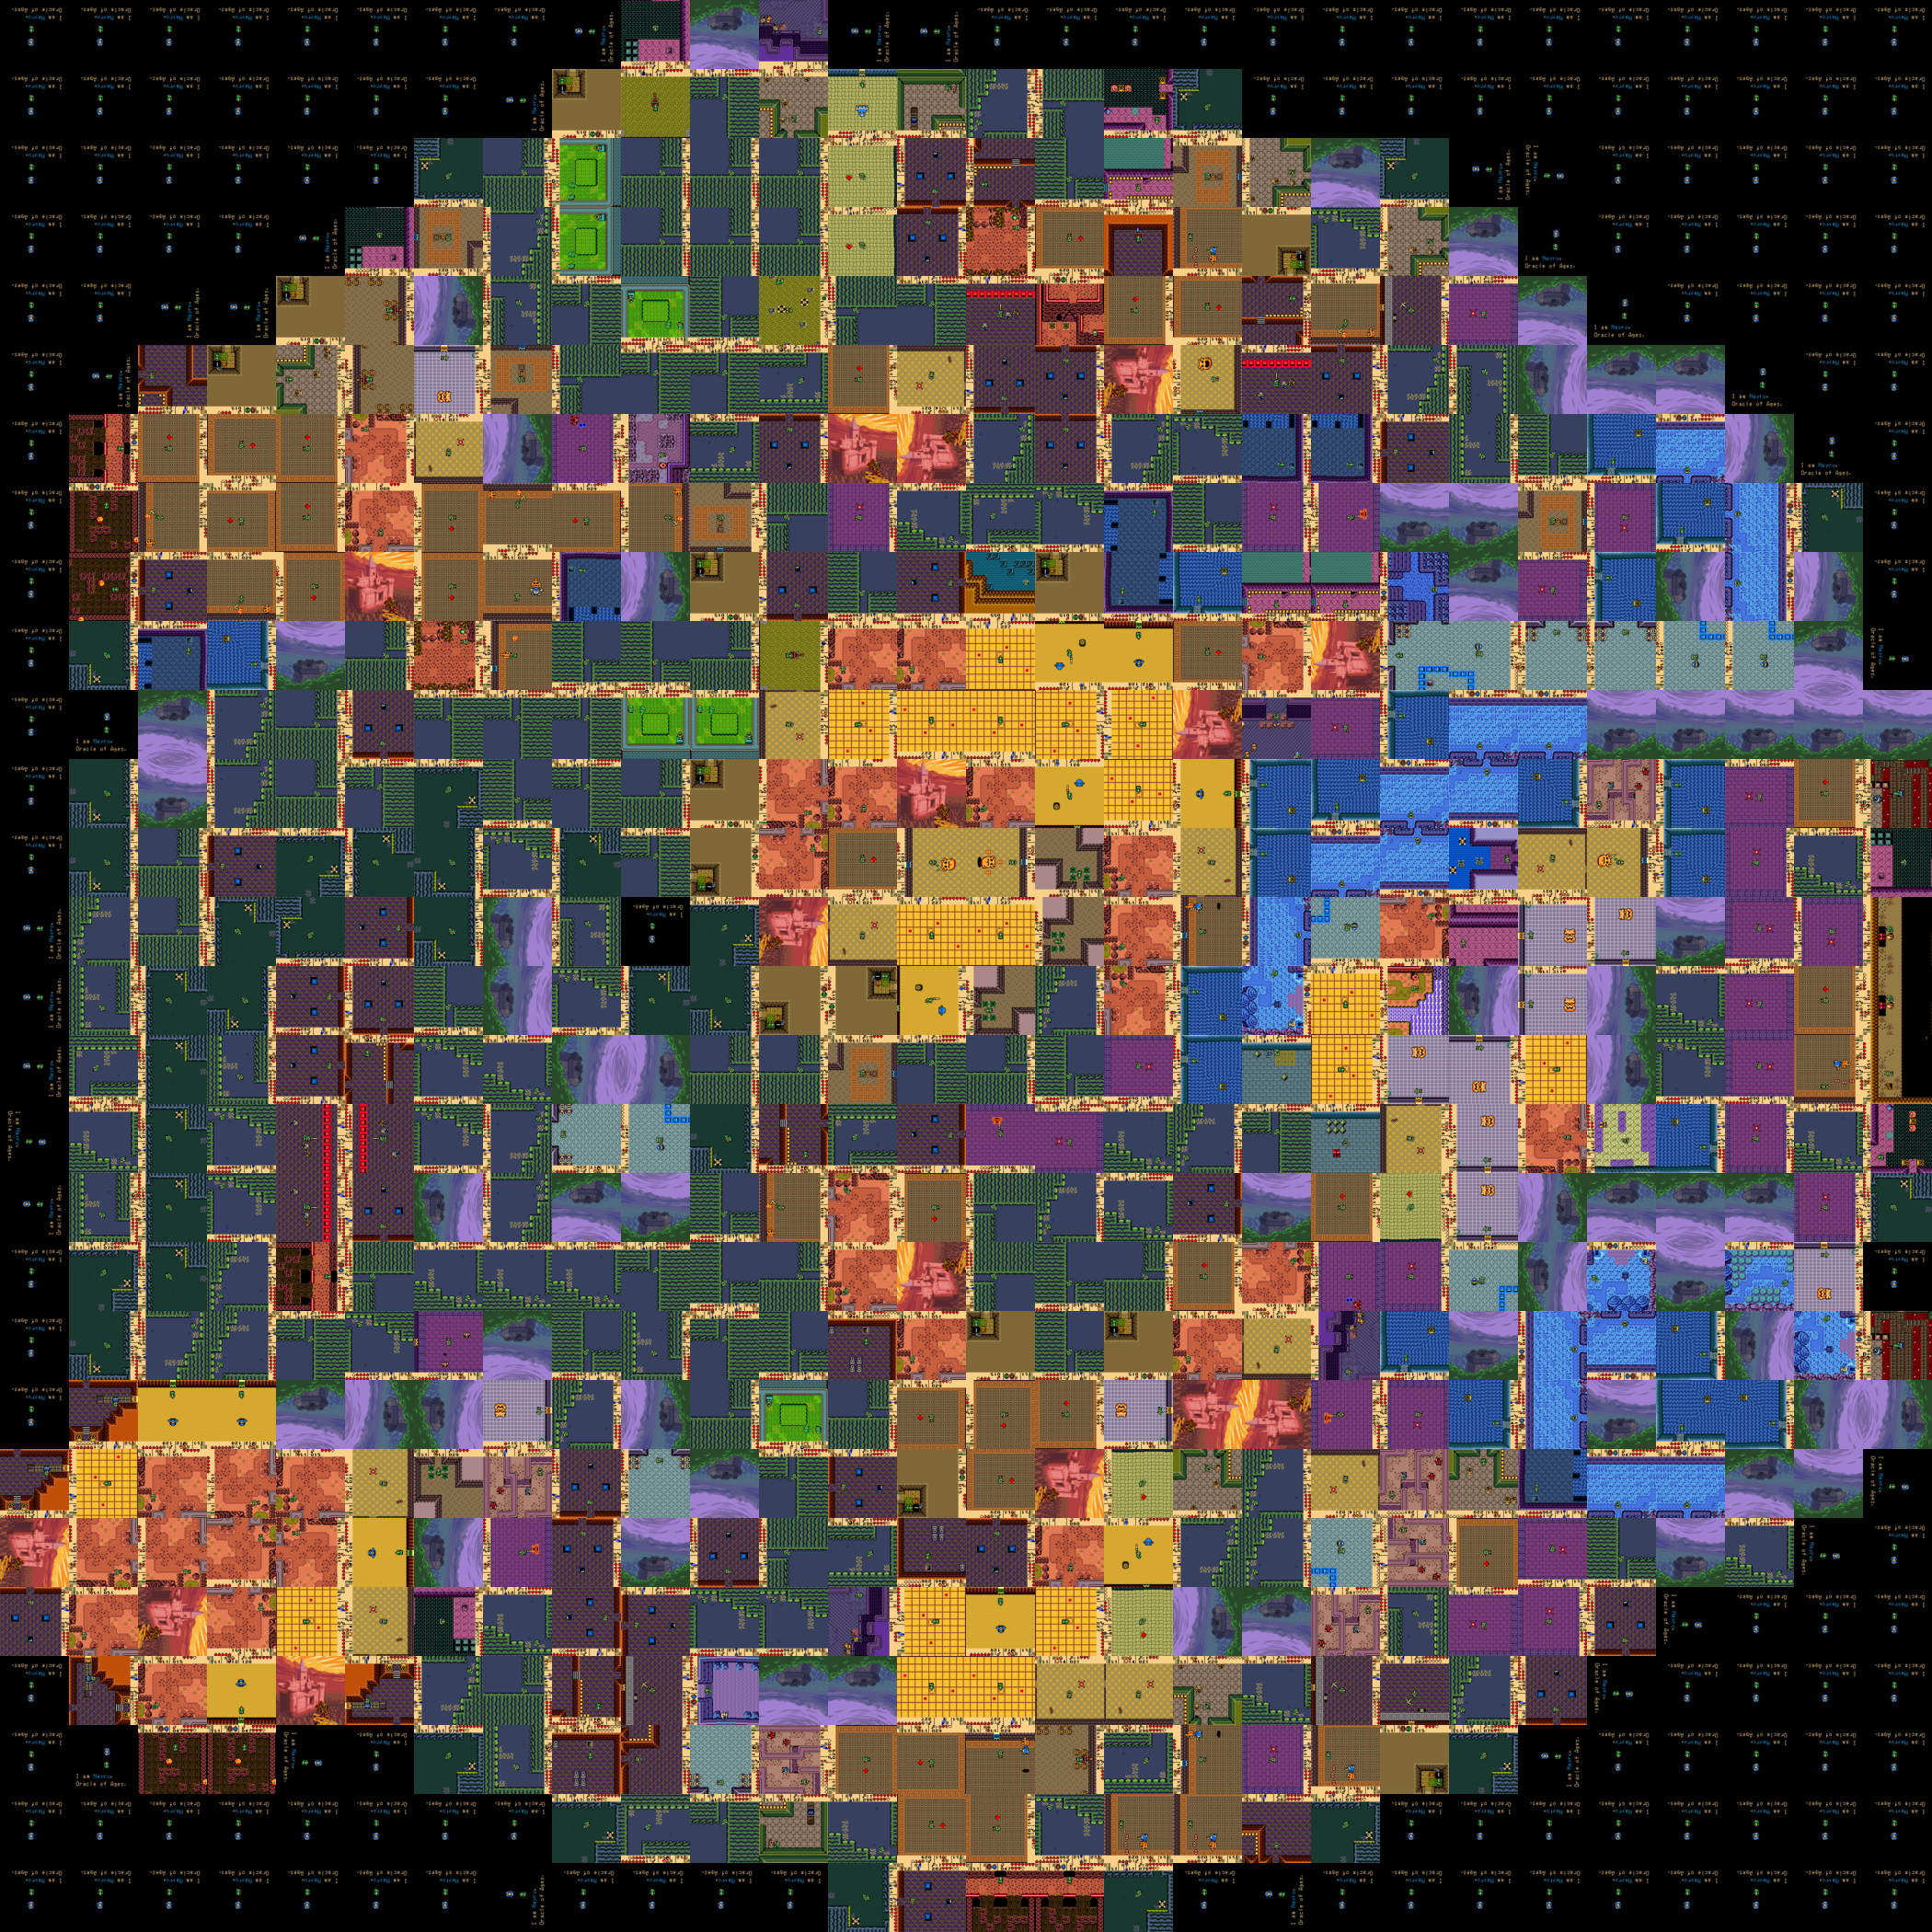
\includegraphics[width=\linewidth]{img/oracle_of_ages_v1.png}
        \caption{Version 1 Mosaic}
    \end{subfigure}
    \begin{subfigure}{0.35\textwidth}
        \includegraphics[width=\linewidth]{img/oracle_of_ages_v2.png}
        \caption{Version 2 Mosaic}
    \end{subfigure}
    \begin{subfigure}{0.35\textwidth}
        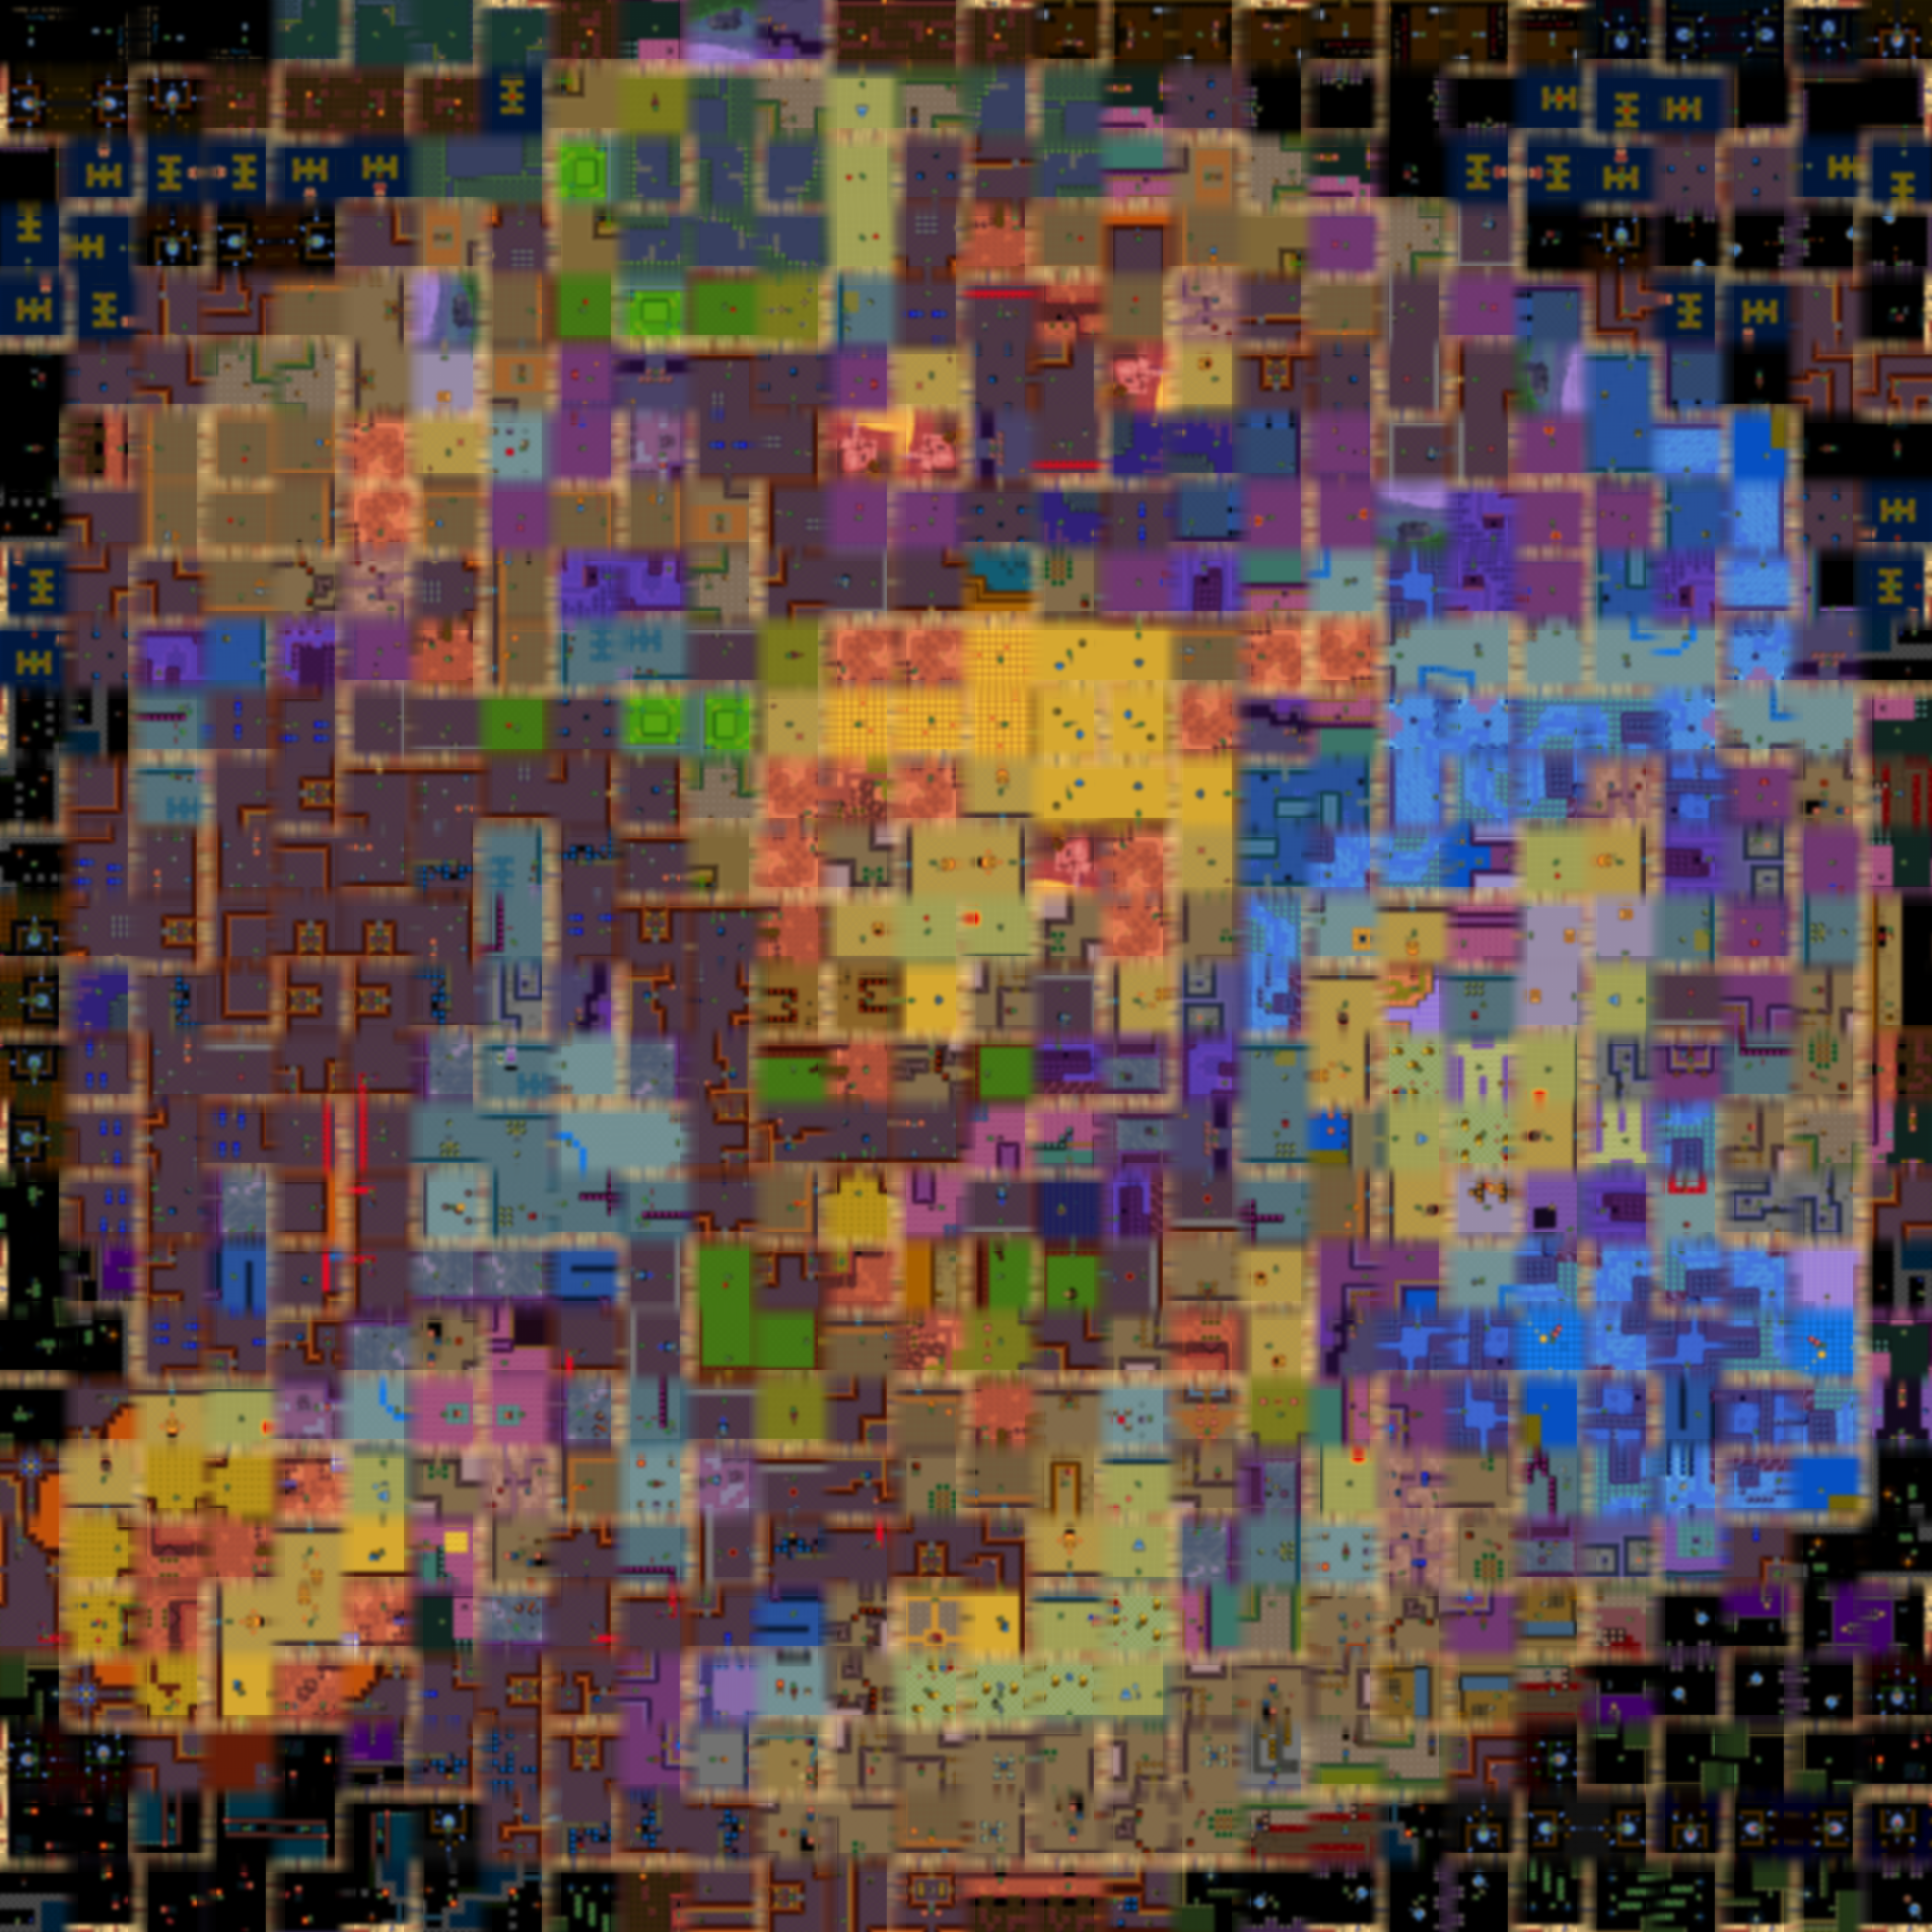
\includegraphics[width=\linewidth]{img/oracle_of_ages_v3.png}
        \caption{Version 3 Mosaic}
    \end{subfigure}
    \begin{subfigure}{0.35\textwidth}
        
\includegraphics[width=\linewidth]{img/oracle_of_ages_v1_smaller.png}
        \caption{Version 1 Mosaic with smaller inputs}
    \end{subfigure}
    \begin{subfigure}{0.35\textwidth}
        \includegraphics[width=\linewidth]{img/oracle_of_ages_v3_smaller.png}
        \caption{Version 3 Mosaic with smaller inputs}
    \end{subfigure}
    \caption{\texttt{zelda-mosaic} sample}\label{F:zelda-mosaic-sample}
\end{figure*}

We iteratively developed three versions after our initial proof-of-concept. Each
version refines the algorithm of the previous version (for details, the
pseudocode for each algorithm may be found in
\figurename{s}~\ref{alg:v1},~\ref{alg:v2}, and~\ref{alg:v3}). We also further
refined mosaic quality by stitching smaller images, at a performance cost. The
original presentation is publicly available~\cite{zelda_mosaic_pres}, as is a
separate video-recording~\cite{zelda_mosaic_vid}.

Our original goal was to examine these algorithms as implemented in the \matlab\
source and prove, if possible, their termination given well-conditioned input.
With some of the work now behind us, we have a better idea of what this project
entails and how we will be able to reach the finish line.

\section{Progress Report}

The starting point to our project was to fill in some knowledge gaps that we had
not covered in class prior to when we began. Since we planned to model a
program, we needed to know more about the modeling of programs and execution. To
this end, we completed work in \textit{Software Foundations} up to the chapter
\textit{Simple Imperative Programs}~\cite{Pierce:SF1}. This chapter provided
great insight on how to model statements and expressions, maintain state over a
program's execution, and define semantics. After completing this, we were better
able to outline the scope of the project.

Our progress thus far can be divided into two main categories:
\begin{inlist}
\item determining the subset of \matlab\ (dubbed \mmatlab) relevant to our program, and
\item creating data structures and functions suitable to model the behaviors of
    \mmatlab\@.
\end{inlist}

We also identify two main future tasks that will rely upon the completion of
these tasks:
\begin{inlist}
\item binding operations from the \mmatlab\ language to semantics in
    Coq~\cite{Coq}, and
\item using Hoare logic~\cite{Hoare_1969} to prove that the program terminates
    under what pre-conditions.
\end{inlist}

\subsection{\mmatlab}\label{S:mmatlab}

We give a brief overview on \mmatlab, the subset of \matlab\ that we model in
order to prove facts about our programs.

Aside from general programming patterns for control flow, the main syntax of
relevance in our program involves array/matrix accesses and updates, arithmetic
operations, and \matlab-specific primitives such as ranges. We have identified
all of the expressions and statements we expect to use and defined them as
inductive types, shown in \figurename~\ref{fig:inductivetypeexp} and
\figurename~\ref{fig:inductivetypestmt}.

\begin{figure}[ht]
    \centering
    \begin{align*}
        \mathsf{exp} \triangleq\;
        & |\; \mathsf{IntLiteral} \\
        & |\; \mathsf{FloatLiteral} \\
        & |\; \mathsf{AddExp} \\
        & |\; \mathsf{MultExp} \\
        & |\; \mathsf{DivExp} \\
        & |\; \mathsf{EqualsExp} \\
        & |\; \mathsf{NotEqualsExp} \\
        & |\; \mathsf{LTEqualsExp} \\
        & |\; \mathsf{Floor} \\
        & |\; \mathsf{VarRefExp} \\
        & |\; \mathsf{RangeExp} \\
        & |\; \mathsf{MatrixLiteral} \\
        & |\; \mathsf{IndexExp} \\
        & |\; \mathsf{SqueezeExpr} \\
        & |\; \mathsf{SizeExpr} \\
        & |\; \mathsf{LengthExpr} \\
        & |\; \mathsf{ProdExpr} \\
        & |\; \mathsf{SumExpr} \\
        & |\; \mathsf{MinExpr} \\
        & |\; \mathsf{MaxExpr} \\
        & |\; \mathsf{PointWiseExpExp} \\
        & |\; \mathsf{ZerosExp} \\
        & |\; \mathsf{OnesExp} \\
        & |\; \mathsf{InfExp} \\
        & |\; \mathsf{FindExp}
    \end{align*}
    \caption{Skeleton of abstract syntax for expressions used in
    \mmatlab\@.}\label{fig:inductivetypeexp}
\end{figure}

\begin{figure}[ht]
    \centering
    \begin{align*}
        \mathsf{statement} \triangleq\;
        & |\; \mathsf{NoOp} \\
        & |\; \mathsf{Error} \\
        & |\; \mathsf{ExprS} \\
        & |\; \mathsf{AssignS} \\
        & |\; \mathsf{IndexedAssignS} \\
        & |\; \mathsf{SeqS} \\
        & |\; \mathsf{WhileS} \\
        & |\; \mathsf{IfThenElseS} \\
    \end{align*}
    \caption{Skeleton of abstract syntax for statements used in
    \mmatlab\@.}\label{fig:inductivetypestmt}
\end{figure}

Much of the abstract syntax is relatively self-explanatory, so complete
definitions are elided here. However, we wish to draw attention to some of the
less apparent and more interesting syntax present in \mmatlab\@:

\begin{itemize}

    \item \textsf{AddExp}: While this is nominally a regular addition operator,
        \matlab's addition is interesting in that it has overloaded parameter
        types and expected behavior for each. The addition of two numbers is a
        number and the addition of two matrices results in element-wise
        addition, as one might expect. However, the sum of a number and a
        matrix, is a matrix with all elements incremented by the number. Similar
        behaviors hold for \textsf{MultExp} and \textsf{DivExp}.

    \item \textsf{RangeExp}: Like Python, \matlab\ has an expression where a
        starting number and stopping number may be provided, generating an
        inclusive list of all numbers between them.

    \item \textsf{SqueezeExpr}: For multi-dimensional arrays, sometimes the size
        of a particular dimension will be 1. \texttt{squeeze} is a function that
        reduces dimensionality by discarding or ``squeezing'' these superfluous
        dimensions.

\end{itemize}

\subsection{Data Structures and Functions}

Our program is used for image processing; thus, many computations are made on
images, which are represented as arrays in \matlab\@. Additionally, we deal with
matrices of images, so we need to model multi-dimensional matrices. Since
multi-dimensional matrices can have arbitrarily many dimensions, we decided the
best abstraction for this in Coq would be built on top of the \textsf{Vector}
type which was originally implemented in the \colorlib\
library~\cite{BLANQUI_2011} and eventually ported to the Coq standard library.
In Coq, \textsf{Vector} is a dependent type~\cite{Bove2009,Thorsten_2010}; the
number of elements in a \textsf{Vector} is part of its type, written
\texttt{Vector.t A n} for a vector containing \(n\) elements of type \(A\).
Since \textsf{Vector}s are polymorphic, we noted that a \textsf{Vector} could
contain \textsf{Vector}s provided they are all the same type (which includes
length, as noted). That is, we can stack \textsf{Vector}s to form, \emph{e.g.},
\texttt{Vector.t (Vector.t A m) n}. From there, we defined a type-constructor
\textsf{Matrix} taking a list of dimensions, which represents a \textsf{Vector}
of \textsf{Vector}s. It can be used as the type of an arbitrary
\(n\)-dimensional matrix containing elements of type \(A\).

Due to the implementation of \textsf{Vector} in the Coq standard library, we
needed to greatly extend the functionality of our \textsf{Matrix} type. To that
end, we have begun implementing \textsf{Matrix} functions such as element
access, which is non-trivial for matrices with an arbitrary number of
dimensions\footnote{In particular because of the dependent types; see also
\url{https://stackoverflow.com/q/66863226/4400820}}. Additionally, the existing
implementation of element access in Coq's \textsf{Vector} type uses the
unfamiliar \textsf{Fin} type, an abstraction for carrying proofs that a
particular number belongs to finite range of numbers. In order to access an
element of a \textsf{Vector}, one must supply such a proof; for our purposes, we
use \texttt{Fin.of\_nat}, which gives either such a proof or a witness that the
number is outside the range. This behavior is captured by the \textsf{sumbool}
built-in, which required further research on our behalf. Given the number of
ways that matrices can be indexed in \matlab\ and the complexity introduced by
Coq's implementation of \textsf{Vector}s, we see this as the main bottleneck for
our progress. We still need to implement many \textsf{Matrix} operations, such
as accesses over ranges and over an entire dimension.

\subsection{Binding Operations and Semantics}

While we have not yet bound any of our functions or data types to the statements
or expressions in \S~\ref{S:mmatlab}, we have naturally been thinking about them
throughout the whole process. The functions we write are intended to implement
the evaluation of the corresponding expressions. In the style of
\texttt{Imp}~\cite{Pierce:SF1}, we intend to write a deterministic expression
evaluation function; we will then provide semantics for program execution.
Execution cannot be defined as a function in Coq because it may be
non-terminating. We have had to consider what operations are be allowed and
whether checks for undesired behavior (\emph{e.g.}, dynamic type mismatches)
should be implemented in the underlying functions or in a semantic check.

\subsection{Hoare Logic}

We have a significant amount of work to do in modeling \mmatlab, but the
blue-sky goal remains to prove the termination of our program given that certain
preconditions hold. Ben has been studying Hoare logic~\cite{Hoare_1969}, the
relevant background material for this problem, as part of his Thesis
requirement. What will be possible to prove will be determined in part by what
we are able to successfully model, given the time constraints. However, as a
preliminary step, we have studied partial Hoare logic and total Hoare logic to
provide more context for the task ahead of us. In this exploration, we found
that partial Hoare logic is a weak statement about programs; namely, given
preconditions \(P\) and postconditions \(Q\) and a program \(C\), the Hoare
triple \(\{P\}C\{Q\}\) asserts that \emph{if} \(C\) terminates, then the
pre-conditions imply the post-conditions. Total Hoare logic, by contrast, is a
stronger version of this claim: \(C\) is asserted to terminate. Thus a proof in
total Hoare logic necessitates a proof that \(C\) terminates; the inference
rules are accordingly adjusted. The primary adjustment is to the rule for while
loops, which are guaranteed to terminate by relation to a decreasing sequence
(with respect to a well-founded order). Given that we are trying to prove
termination, it seems likely that we will need to use total Hoare logic in the
relevant proofs.

\begin{figure}[ht]
    \textbf{Input}: image \(key\_art\), images \(thumbnails\), integer \(size\) \\
    \textbf{Output}: image \(tiles\)
    \begin{algorithmic}
        \STATE{\(tiles \gets \textrm{MAT2TILES}(key\_art, size, size)\)}
        \FOR{\(tile \in tiles\)}
            \FOR{\(thumbnail, i \in thumbnails, [1..|thumbnails|]\)}
                \STATE{\(mses_i \gets \textrm{immse}(tile, thumbnail)\)}
            \ENDFOR
            \STATE{\(best\_indices \gets \textrm{find} (mses = \min mses)\)}
            \STATE{\(best\_index \gets best\_indices_0\)}
            \STATE{\(tile \gets thumbnails_{best\_index}\)}
        \ENDFOR
    \RETURN{\(tiles\)}
    \end{algorithmic}
    \caption{Algorithm: Version 1}\label{alg:v1}
\end{figure}

\begin{figure}[ht]
    \textbf{Input}: image \(key\_art\), images \(thumbnails\), integer \(size\) \\
    \textbf{Output}: image \(tiles\)
    \begin{algorithmic}
        \STATE{\(tiles \gets \textrm{MAT2TILES}(key\_art, size, size)\)}
        \STATE{\(used \gets \emptyset\)}
        \STATE{\(threshold \gets 1\)}
        \IF{\(|thumbnails| < |tiles|\)}
            \STATE{\(threshold \gets \lceil{|tiles| / |thumbnails|}\rceil\)}
        \ENDIF
        \FOR{\(tile \in tiles\)}
            \FOR{\(thumbnail, i \in thumbnails, [1..|thumbnails|]\)}
                \STATE{\(mses_i \gets \textrm{immse}(tile, thumbnail)\)}
            \ENDFOR
            \STATE{\(best\_indices \gets \textrm{find} (mses = \min mses)\)}
            \STATE{\(best\_index \gets best\_indices_0\)}
            \WHILE{\(used_{best\_index} \ge threshold\)}
                \STATE{\(mses_{best\_index} \gets \infty\)}
                \STATE{\(best\_indices \gets \textrm{find} (mses = \min mses)\)}
                \STATE{\(best\_index \gets best\_indices_0\)}
            \ENDWHILE
            \STATE{increment \(used_{best\_index}\)}
            \STATE{\(tile \gets thumbnails_{best\_index}\)}
        \ENDFOR
        \RETURN{\(tiles\)}
    \end{algorithmic}
    \caption{Algorithm: Version 2}\label{alg:v2}
\end{figure}

\begin{figure}[ht]
    \textbf{Input}: image \(key\_art\), images \(thumbnails\), integer \(size\) \\
    \textbf{Output}: image \(tiles\)
    \begin{algorithmic}
        \STATE{}\COMMENT{Repeat Version 2}
        \STATE{\(tiles \gets \textrm{Version2}(key\_art, thumbnails, size)\)}
        \STATE{\(tiles \gets \textrm{imgaussfilt}(tiles)\)}
        \STATE{\(strip\_size \gets \lfloor{size / 8}\rfloor\)}
        \STATE{}\COMMENT{Blur by averaging}
        \FOR{horizontal \(strip \in tiles\)}
            \STATE{\(strip \gets \textrm{mean}({strip})\)}
        \ENDFOR
        \FOR{vertical \(strip \in tiles\)}
            \STATE{\(strip \gets \textrm{mean}({strip})\)}
        \ENDFOR
        \RETURN{\(tiles\)}
    \end{algorithmic}
    \caption{Algorithm: Version 3}\label{alg:v3}
\end{figure}

{\printbibliography}

\end{document}
